\documentclass[12pt,letterpaper]{article}
\usepackage{graphicx,textcomp}
\usepackage{natbib}
\usepackage{setspace}
\usepackage{fullpage}
\usepackage{color}
\usepackage[reqno]{amsmath}
\usepackage{amsthm}
\usepackage{fancyvrb}
\usepackage{amssymb,enumerate}
\usepackage[all]{xy}
\usepackage{endnotes}
\usepackage{lscape}
\newtheorem{com}{Comment}
\usepackage{float}
\usepackage{hyperref}
\newtheorem{lem} {Lemma}
\newtheorem{prop}{Proposition}
\newtheorem{thm}{Theorem}
\newtheorem{defn}{Definition}
\newtheorem{cor}{Corollary}
\newtheorem{obs}{Observation}
\usepackage[compact]{titlesec}
\usepackage{dcolumn}
\usepackage{tikz}
\usetikzlibrary{arrows}
\usepackage{multirow}
\usepackage{xcolor}
\newcolumntype{.}{D{.}{.}{-1}}
\newcolumntype{d}[1]{D{.}{.}{#1}}
\definecolor{light-gray}{gray}{0.65}
\usepackage{url}
\usepackage{listings}
\usepackage{color}
 
\definecolor{codegreen}{rgb}{0,0.6,0}
\definecolor{codegray}{rgb}{0.5,0.5,0.5}
\definecolor{codepurple}{rgb}{0.58,0,0.82}
\definecolor{backcolour}{rgb}{0.95,0.95,0.92}
 
\lstdefinestyle{mystyle}{
    backgroundcolor=\color{backcolour},   
    commentstyle=\color{codegreen},
    keywordstyle=\color{magenta},
    numberstyle=\tiny\color{codegray},
    stringstyle=\color{codepurple},
    basicstyle=\footnotesize,
    breakatwhitespace=false,         
    breaklines=true,                 
    captionpos=b,                    
    keepspaces=true,                 
    numbers=left,                    
    numbersep=5pt,                  
    showspaces=false,                
    showstringspaces=false,
    showtabs=false,                  
    tabsize=2
}
 \lstset{style=mystyle}
\newcommand{\Sref}[1]{Section~\ref{#1}}
\newtheorem{hyp}{Hypothesis}

\title{Network Analysis: Homework}
\date{Due: August 23, 2018}
\author{Jeff Ziegler}

\begin{document}
\maketitle

\section{Nigeria Data Processing}

\begin{itemize}
	\item[a)] Process the data: turn this event dataset into a matrix.
	\item[b)] Specifically, summarize the interactions across all time periods into an adjacency matrix where:
	\begin{enumerate}
		\item "1" indicates that $i$ and $j$ had a conflictual interaction sometime during the temporal span of the original dataset and zero otherwise.
		\item Make sure all actors that existed at any point during the temporal span are included in the adjacency matrix.
	\end{enumerate}
\end{itemize}

	\lstinputlisting[language=R, firstline=1, lastline=38]{JZ_Homework.r}  
	
\section{Measurements \& Community Detection}

\begin{itemize}
	\item[a)] Which actor is the most “influential” in the network? Justify your response and the measure you choose to estimate “influence.”
	\item[b)] Employ the blockmodel function from the sna package to explore potential group level structure in the data (see slides 61-63 from day 2 for details):
	\begin{itemize}
		\item Run blockmodel with varying levels of k.
		\item Save the node classifications from each run.
		\item Now how do we choose k?
			\begin{itemize}
				\item You will do so through an out-of-sample cross-validation exercise (at least 10 folds).
				\item Report the AUC (ROC) and AUC (PR) statistics from each model.
			\end{itemize}
	\end{itemize}
	\item [c)] After having determined the k that gives the best out of sample performance, visualize your results as shown in slide 67 from the day 2 lecture
\end{itemize}

\lstinputlisting[language=R, firstline=40, lastline=153]{JZ_Homework.r}  

\begin{verbatim}
k   AUC_ROC     AUC_PR
1  2 0.5321138 0.07721483
2  3 0.5245793 0.07547592
3  4 0.5420858 0.07672680
4  5 0.5394230 0.08071837
5  6 0.5424247 0.07655145
6  7 0.5628951 0.08848244
7  8 0.5366850 0.08067494
8  9 0.5243585 0.07983234
9 10 0.5489216 0.08615140
\end{verbatim}

\lstinputlisting[language=R, firstline=155, lastline=175]{JZ_Homework.r}  

\begin{figure}[h!]\centering
	\caption{\footnotesize{Network plot by groups generated from block model with 7 clusters.}}\label{fig:figure1}
	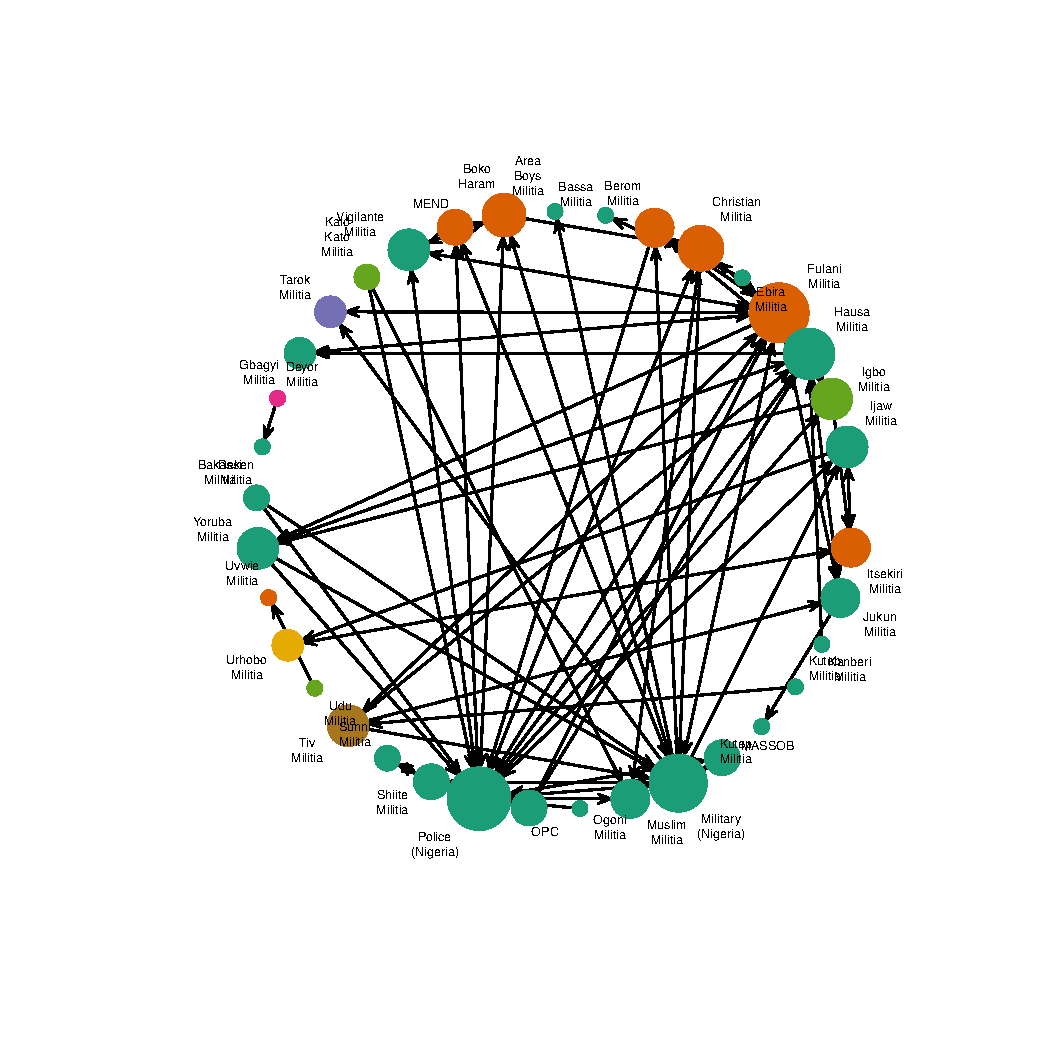
\includegraphics[width=.99\textwidth]{figure1.pdf}\\
\end{figure}

\section{ERGMs}

\begin{itemize}
	\item[a)] Run a cross-sectional ERGM on the Nigerian conflict network, develop at least one or two network level hypotheses.
	\item[b)] Briefly discuss the results.
	\item [c)] Make sure to show that you checked for convergence.
\end{itemize}

\lstinputlisting[language=R, firstline=177,lastline=400]{JZ_Homework.r}  

\begin{verbatim}
Monte Carlo MLE Results:
Estimate Std. Error MCMC % z value Pr(>|z|)    
edges   -3.4543     0.1653      0   -20.9   <1e-04 ***
mutual   3.8490     0.3738      0    10.3   <1e-04 ***
---
Signif. codes:  0 ‘***’ 0.001 ‘**’ 0.01 ‘*’ 0.05 ‘.’ 0.1 ‘ ’ 1
\end{verbatim}

\begin{figure}[h!]\centering
	\caption{\footnotesize{MCMC chain and estimate distribution.}}\label{fig:figure2}
	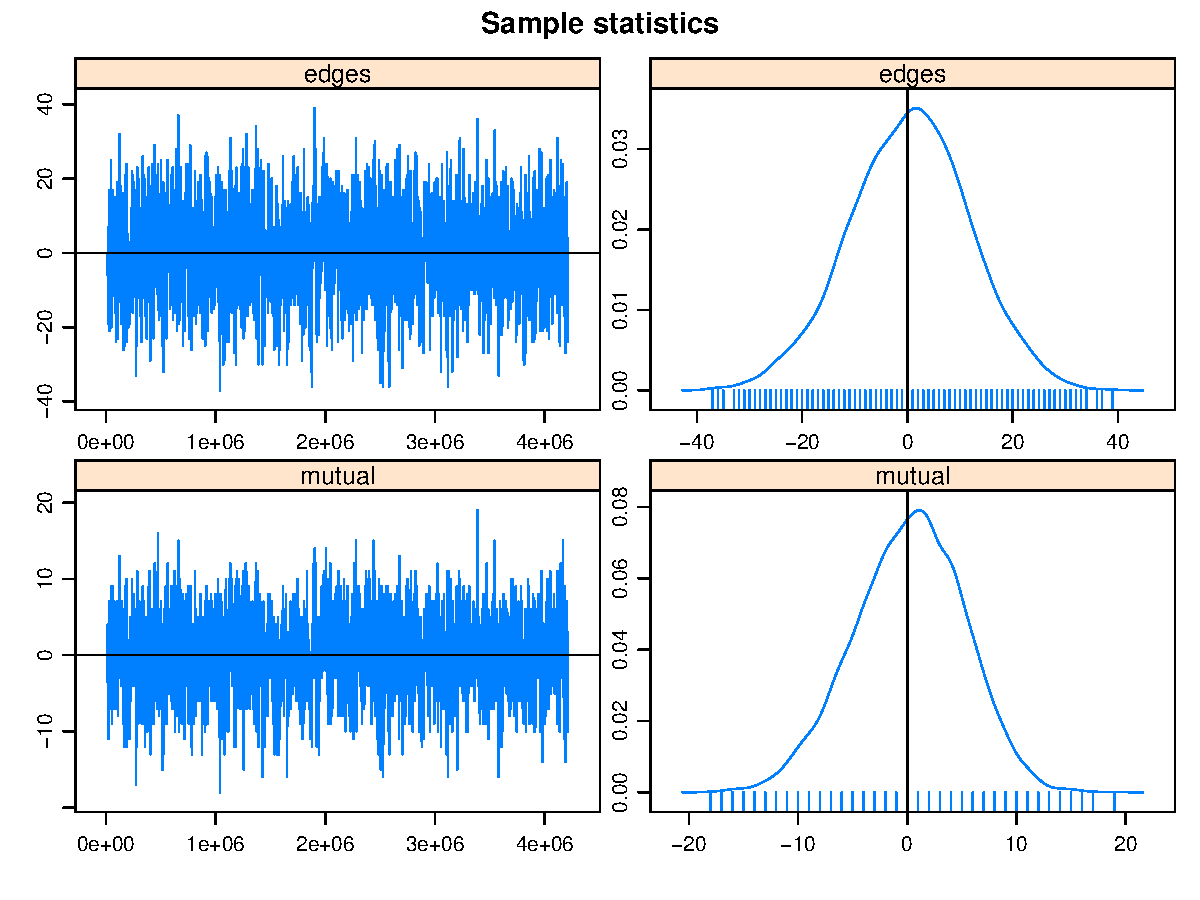
\includegraphics[width=.7\textwidth]{figure2.pdf}\\
\end{figure}

\section{Find your own data}

\begin{itemize}
	\item[a)] Locate data that relates to your field of interest.
	\item[b)] Transform the data, or a subset of it into a matrix, and plot (similar to step 1 in Section 1).
	\item [c)] Include descriptive features in your network graph (similar to step 2, but choose your own measurements).
	\item [d)] Run a model, it can be any network model from the course but justify your choices! 
	\item [e)] Discuss the results in a brief write up. Present for 3-5 minutes to the class.
\end{itemize}

\lstinputlisting[language=R, firstline=26,lastline=400]{JZ_BITs.r}  

\end{document}
